\documentclass{beamer}

\usetheme{metropolis}

\usepackage[style=numeric,sorting=ynt]{biblatex}
\usepackage[localise]{xepersian}

\setlatintextfont{Roboto}

\settextfont{Vazir}


% ---------------------------------------------------------------------------------
% Colors
% ---------------------------------------------------------------------------------
\definecolor{نارنجی}{rgb}{1.0, 0.31, 0.0}

% ---------------------------------------------------------------------------------
% Settings to force Beamer works with Xepersian and RTL typesetting
% ---------------------------------------------------------------------------------
% \raggedleft

% For right to left lists (itemize and enumerate)
\makeatletter
\newcommand{\لیست‌فارسی}{\raggedleft\rightskip\@totalleftmargin}
\makeatother
% Correct the bullet for RTL texts
\setbeamertemplate{itemize item}{\scriptsize\raise1.25pt%
  \hbox{\donotcoloroutermaths$\blacktriangleleft$}}

% To force beamer use numbering in captions
\setbeamertemplate{caption}[numbered]{}% Number float-like environments

\setbeamertemplate{footline}[frame number]
\setbeamertemplate{section in toc}[circle]
\setbeamercolor{block body}{bg=lightgray}
\setbeamercolor{headline}{bg=orange}
\setbeamersize{text margin left=1cm,text margin right=1cm}

\setbeamertemplate{headline}
{
  \begin{beamercolorbox}{section in head/foot}
    \vspace{2pt}\insertnavigation{\paperwidth}\vspace{2pt}
  \end{beamercolorbox}
}

% ---------------------------------------------------------------------------------
% To force beamer use numbering in captions
\setbeamertemplate{caption}[numbered]{}% Number float-like environments

\setbeamertemplate{footline}
{%
  \leavevmode%
  \hbox{%
    \begin{beamercolorbox}[wd=.333333\paperwidth,ht=2.25ex,dp=1ex,center]{author in head/foot}%
      \usebeamerfont{author in head/foot}\insertshortauthor%
    \end{beamercolorbox}%
    \begin{beamercolorbox}[wd=.333333\paperwidth,ht=2.25ex,dp=1ex,center]{title in head/foot}%
      \usebeamerfont{title in head/foot}\insertshorttitle%
    \end{beamercolorbox}%
    \begin{beamercolorbox}[wd=.333333\paperwidth,ht=2.25ex,dp=1ex,right]{date in head/foot}%
      \usebeamerfont{date in head/foot}\insertsection\hspace*{2em}
      \insertframenumber~ از \inserttotalframenumber{} \hspace*{2ex}%
    \end{beamercolorbox}
  }%
}
\setbeamertemplate{section in toc}[circle]
\setbeamertemplate{blocks}[rounded][shadow=false]
\setbeamercolor{block title}{bg=orange}
\setbeamercolor{block body}{bg=lightgray}
\setbeamersize{text margin left=1cm,text margin right=1cm}
\setbeamertemplate{frametitle continuation}{\insertcontinuationcount}

\author[الهه داستان]{%
  الهه داستان\hfill
  ۹۶۳۱۰۲۵\\
}
\title{پیش‌بینی ترافیک به وسیله شبکه‌های عصبی}
\subtitle{%
  پروژه کارشناسی\\
  دکتر صفابخش
}
\institute[]{دانشگاه صنعتی امیرکبیر}
\date{زمستان ۱۴۰۰}

\AtBeginSection[]
{
  \begin{frame}
    \frametitle{فهرست}
    \tableofcontents[currentsection]
  \end{frame}
}

\addbibresource{main.bib}

\begin{document}

\begin{persian}

\begin{frame}
  \titlepage{}
\end{frame}

\begin{frame}
  \frametitle{فهرست}
  \tableofcontents{}
\end{frame}

\section{مقدمه}

\begin{frame}
  \frametitle{هدف نهایی}
  \begin{block}{}
    مسافرت از یک نقطه مبدا تا یک نقطه مقصد چقدر طول می‌کشد؟
  \end{block}
\end{frame}

\begin{frame}
  \frametitle{هدف}
  \begin{columns}
    \column{.5\textwidth}
    \begin{block}{تعریف}
      پیش‌بینی سرعت در یک نقطه جغرافیایی مشخص در یک زمان مشخص
    \end{block}
    \pause
    \begin{block}{مثال}
      assume you want to go to the university and you want to know the speed of traffic at Theater Shahr on sunday at 9 am.
    \end{block}
    \pause
    \column{.45\textwidth}
    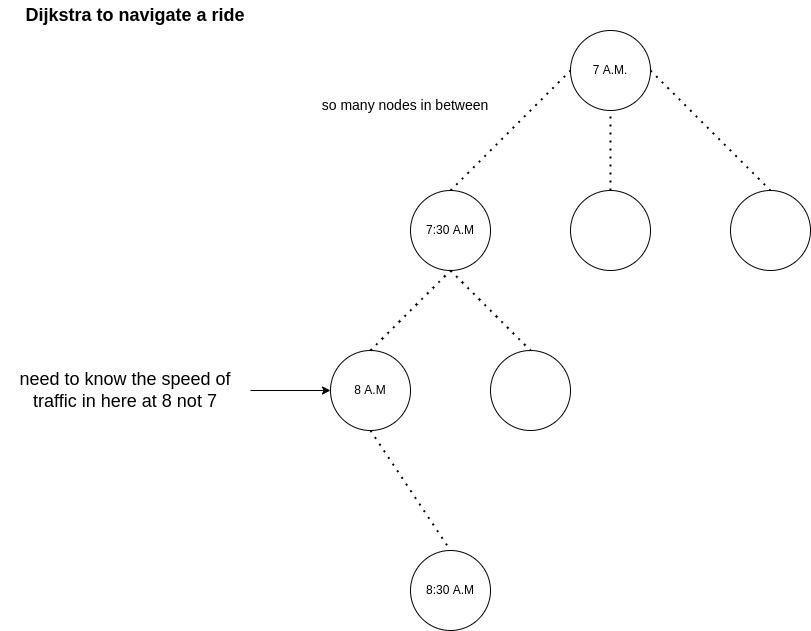
\includegraphics[height=0.5\textheight]{./img/dijkstra.png}
  \end{columns}
\end{frame}

\begin{frame}
  \frametitle{چه کسانی به آن احتیاج دارند؟}
  \begin{columns}
    \column{.25\textwidth}
    
\includegraphics[height=0.5\textheight]{./img/google-maps.png}
    \textbf{Google Maps}\\
    \textit{Google}
    \column{.25\textwidth}
    
\includegraphics[height=0.5\textheight]{./img/waze.png}
    \textbf{Waze}\\
    \textit{Google}
    \column{.25\textwidth}
    
\includegraphics[height=0.5\textheight]{./img/balad.png}
    \textbf{Balad}\\
    \textit{Naghshe Pardazan Ertabatat Novin}
    \column{.25\textwidth}
    
\includegraphics[height=0.5\textheight]{./img/neshan.png}
    \textbf{Neshan}\\
    \textit{Neshan Maps Platform}
  \end{columns}
\end{frame}

\begin{frame}
  \frametitle{چالش‌ها\footfullcite{2004.08555}}
  \شروع{فقرات}
  \لیست‌فارسی
  \فقره داده ترافیکی به صورت زمانی-مکانی است.
  \شروع{فقرات}
  \لیست‌فارسی
  \فقره وابستگی‌های مکانی پیچیده
  \فقره وابستگی‌های زمانی پیچیده
  \پایان{فقرات}
  \فقره فاکتورهای خارجی
  \پایان{فقرات}
  \centering
  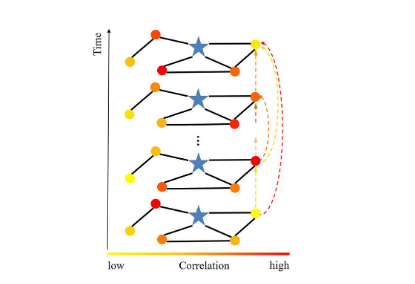
\includegraphics[height=0.5\textheight]{./img/correlations.png}
\end{frame}

\begin{frame}
  \frametitle{تعریف مساله}
  \begin{equation}
    \label{eq:base}
    \hat{v}_{t+1}, \ldots,  \hat{v}_{t+H} = \mathop{\mathrm{argmax}} \log \mathsf{P}({v}_{t+1}, \ldots,  v_{t+H} | v_{t-M+1} , \ldots,  v_{t})
  \end{equation}
  \centering
  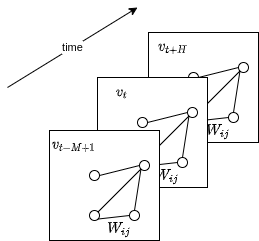
\includegraphics[height=.5\textheight]{img/base.png} % v.drawio
\end{frame}

\begin{frame}
  \frametitle{تعریف گرافی}
  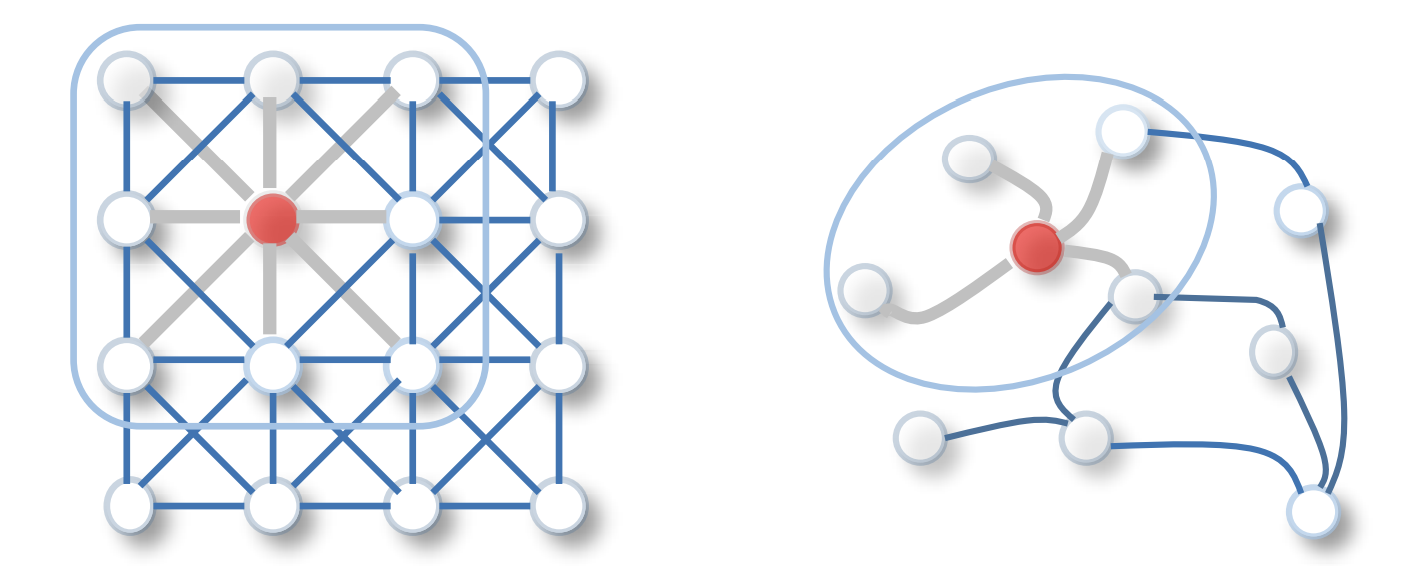
\includegraphics[width=\textwidth]{img/convolution.png}
  \begin{itemize}
    \item با نزدیک شدن گره‌ها به یکدیگر ارتباط میان آن‌ها بیشتر می‌شود
    \item weight matrix dimension is $nxn$
  \end{itemize}
\end{frame}

\section{کارهای مرتبط}

\begin{frame}
  \frametitle{مقدمه\footfullcite{1709.04875}}
  After years of continuous researches, the research on traffic prediction has achieved great progresses.
  \begin{itemize}
    \item traditional methods: Classical Statistical Methods and Machine Learning Methods
    \item deep learning-based methods: Spatial Dependency Modeling and Temporal Dependency Modeling
  \end{itemize}
\end{frame}

\begin{frame}
  \frametitle{کارهای مرتبط}
  \begin{itemize}
  \فقره \متن‌سیاه{مدل خود هم‌بسته میانیگن متحرک}: تنها توالی‌های زمانی را در نظر می‌گیرند.
  \فقره \متن‌سیاه{شبکه باور عمیق}: ویژگی‌های زمانی و مکانی را به صور مشترک سخت از ورودی استخراج می‌کند.
  \فقره \متن‌سیاه{حافظه کوتاه مدت ماندگار}: سنگین از نظر محاسباتی
  \end{itemize}
\end{frame}

\section{راه‌حل پیشنهادی}

\begin{frame}
  \شروع{فقرات}
  \فقره استفاده از هر دو نوع ویژگی زمانی و مکانی
  \فقره در نظر گرفتن مسیرها به صورت گرافی
  \فقره اعمال پیچش به صورت مستقیم بر روی گراف در دامنه طیفی
  \فقره اعمال پیچش بر روی محور زمان
  \پایان{فقرات}
\end{frame}

\begin{frame}
  \frametitle{ورودی راه حل}
  % blackbox
\end{frame}
\begin{frame}
  اطلاعات زمانی
  % v.drawio
\end{frame}
\begin{frame}
  اطلاعات مکانی
  % matrix.drawio
  رابطه اسلاید distance
\end{frame}

\begin{frame}
  \frametitle{Distance}
  \begin{equation}
    W_{i,j} = \left\{
      \begin{array}{ll}
        \exp(-\frac{d^{2}_{ij}}{\sigma^{2}}) & , i \neq j \quad and \quad \exp(-\frac{d^{2}_{ij}}{\sigma^{2}}) \geq \epsilon \\
        0 & , otherwise. \\
      \end{array}\right.
    \label{eq:distance}
  \end{equation}
\end{frame}

\begin{frame}
  \frametitle{Architecture}
  % arch.drawio
\end{frame}

\begin{frame}
  % پیچش در دامنه طیفی
  % رابطه ۴-۲
\end{frame}

\begin{frame}
  \frametitle{Spectral Graph Convolution}
  \begin{equation}
    \Theta *_{g} \chi = \Theta(L)\chi = \Theta(U \Lambda U^{T})\chi = U\Theta(\Lambda)U^{T}\chi
    \label{eq:convolution}
  \end{equation}
  \begin{itemize}
    \item computational complexity is $O(n^{2})$
  \end{itemize}
\end{frame}

\begin{frame}
  \frametitle{Chebyshev Polynomials}
  \begin{equation}
    \Theta \ast_{g} x = \Theta(L)x \approx \sum_{k=0}^{k-1} \Theta_{k} T_{k}(\widetilde{L})x
    \label{eq:approx-convolution}
  \end{equation}
  \begin{itemize}
    \item reduce the complexity
    \item localization
  \end{itemize}
\end{frame}

\begin{frame}
  لایه‌ی پیچشی زمانی
  رابطه ۴-۵
\end{frame}

\begin{frame}
  پیش‌بینی چند گام زمانی آینده
\end{frame}

\section{Datasets and Evaluation}

\begin{frame}
  \frametitle{PeMSD7}
  \begin{itemize}
    \item 228 Nodes
    \item May and June 2012
    \item From sensors
  \end{itemize}
\end{frame}
\begin{frame}
  \frametitle{Snapp}
  \begin{itemize}
    \item GPS Probes
  \end{itemize}
\end{frame}

\begin{frame}[allowframebreaks]
  \frametitle{مراجع}
  \begin{latin}
  \printbibliography[title=مراجع]
  \end{latin}
\end{frame}

\end{persian}

\end{document}
